\section{Volume de billes}


\begin{multicols}{2}
	

Noémie place des billes dans une éprouvette graduée.

\begin{questions}
	\question Quelle est la valeur $V_1$ du volume du tas de billes dans l'éprouvette ? 
	
	\question Elle verse de l'eau dans une éprouvette identique à la précédente. Puis elle verse l'eau dans l'éprouvette contenant les billes. Quel est le volume $V_2$ occupé par les billes ?
	
	\question Comment expliquer la différence entre le volume $V_1$ et le volume $V_2$.
\end{questions}


\begin{center}
	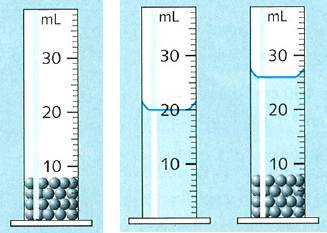
\includegraphics[scale=0.8]{img/billes}
\end{center}
\end{multicols}